\newpage
\section{Du génome aux processus cellulaires}

\subsection{Gènes : Régulations et fonctions}
\label{sec:fn_reg}

Les réactions qui se produisent dans les cellules procaryotes sont souvent complexes et impliquent une multitude de réactifs et de produits. Toutes ces réactions nécessitent la présence de protéines spécifiques pour être réalisées. Ces protéines sont produites et dégradées par la cellule en fonction des conditions rencontrées. C'est pourquoi l'information est stockée dans une structure durable et transmissible, le gène. Chaque gène sera transcrit en une molécule d'ARN messager (ARNm) par l'ARN polymérase, qui sera traduite en protéine par le ribosome (impliquant l'ARNr et l'ARNt). 


Dans une cellule, les protéines ont un temps de "vie" allant de quelques minutes à quelques heures. Il est donc nécessaire de produire les protéines régulièrement, toutefois cette production a un coût pour la cellule. C'est pourquoi il existe des mécanismes de régulation de l'expression des gènes et donc de la production des protéines. Dans la \autoref{sec:gene}, nous avons vu qu'il existait notamment des petits ARN régulateurs de l'expression. Ils agissent en modulant la stabilité ou la traduction des ARN messagers cibles, jouant ainsi un rôle clé dans l’adaptation aux stress environnementaux, la régulation du métabolisme ou encore la virulence par exemple. Dans l'ADN non codant, on retrouve également une séquence promotrice (ou promoteur) près d'un gène qui permet la fixation de l'ARN polymérase. La fixation et l'activation de l'ARN polymérase au niveau du promoteur sont régulées par des facteurs de transcription qui se lient spécifiquement à des séquences régulatrices en amont du promoteur, les \textit{enhancer} et \textit{silencer}.


Les protéines peuvent agir en collaboration, soit dans des réactions successives (cas des systèmes biologiques, cf. \autoref{sec:sys_bio}), soit en formant des complexes protéiques interagissant pour métaboliser un produit. Les gènes codant pour des protéines impliquées dans les mêmes processus cellulaires sont situés dans le même contexte génomique (cf. \autoref{sec:gene}). Ils vont alors être régulés par les mêmes éléments de régulation. L'opéron, une structure spécifique des procaryotes découverte par François Jacob et Jacques Monod en 1960\footnote{Découverte qui leur a valu le prix Nobel de médecine en 1965}\cite{jacob_genetic_1961}, permet de produire un seul ARNm pour un ensemble de gènes codant pour des protéines impliquées dans le même processus cellulaire. Dans l'opéron, se trouve une nouvelle séquence de régulation, l'opérateur, où va se lier une molécule régulatrice qui va activer ou inhiber la transcription (\autoref{fig:lac_operon}). L'ensemble de l'opéron permet de synchroniser la régulation et l'expression de gènes qui collaborent dans le même processus cellulaire.


\begin{figure}[htbp]
    \centering
    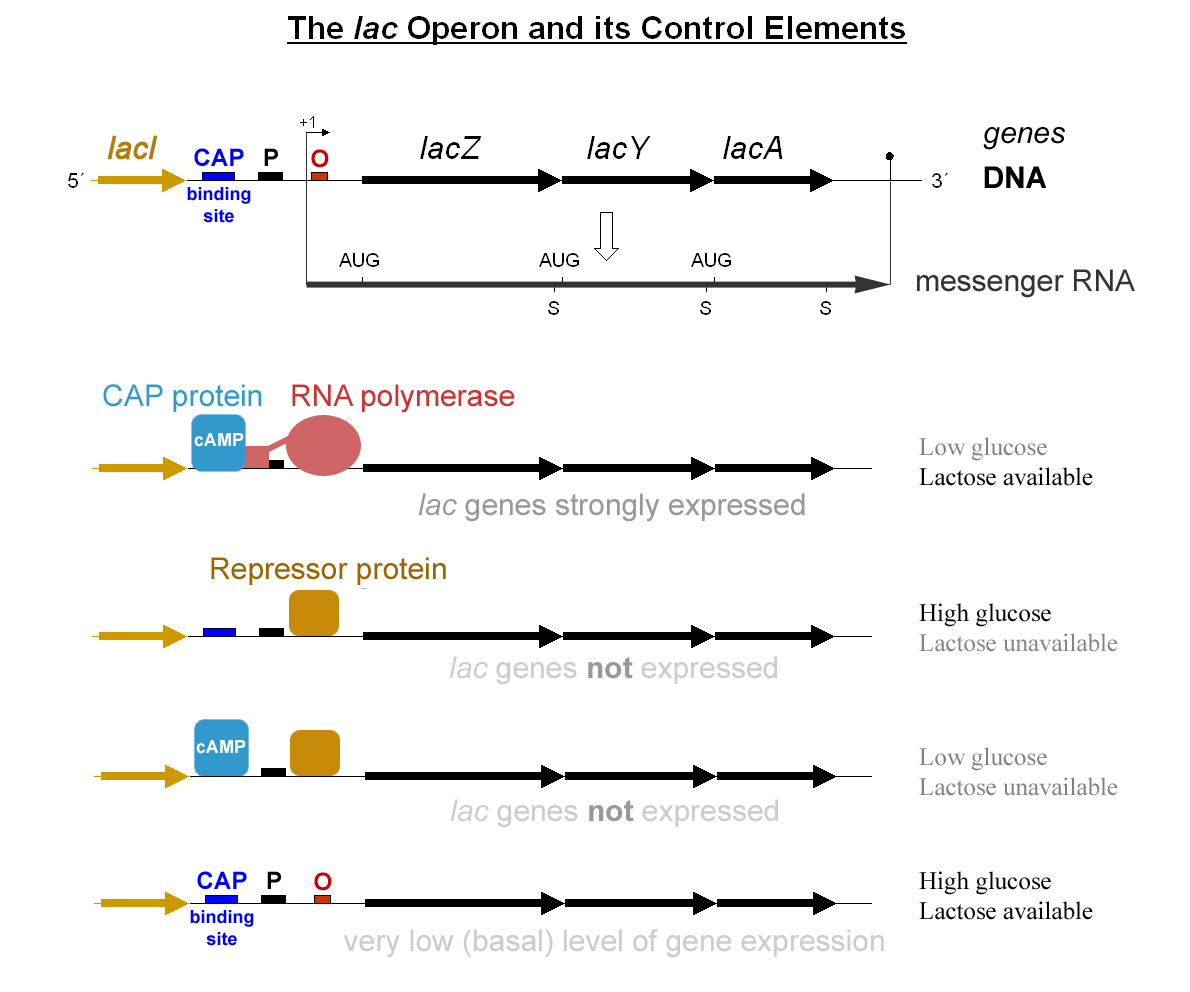
\includegraphics[width=\linewidth]{images/Lac_operon-2010-21-01.png}
    \caption[Exemple de l'opéron lactose]{\textbf{Schéma du fonctionnement de l'opéron lactose.} Sur la partie haute est représenté la structure génétique de l'opéron. Les 4 lignes suivantes représentent chacune une configuration de réponse à des conditions de présence, absence de glucose et de lactose. si le taux de glucose est faible, une protéine activatrice (CAP) va se fixer en amont du promoteur pour aider à la fixation de l'ARN polymérase, et si du lactose est disponible, les gènes seront alors fortement exprimés. Si le lactose n'est pas disponible, une protéine de répression va se fixer à l'opérateur et elle empêchera l'ARN polymérase de se fixer même si le taux de glucose est faible. 
    Auteur : G3pro. Sous licence Creative Commons 2.0. Disponible à l’adresse : \url{https://commons.wikimedia.org/wiki/File:Lac_operon-2010-21-01.png.}
    }
    \label{fig:lac_operon}
\end{figure}

Pour terminer, l'expression des gènes peut aussi être régulée par le niveau de repliement et de condensation de l'ADN. L'ADN est condensé notamment grâce à des protéines spécialisées et à la méthylation de l’ADN. L'ADN replié ne pourra pas être accessible pour la transcription des gènes et donc ils seront inactifs. Les mécanismes liés à la méthylation de l'ADN sont l'affaire de l’épigénétique. Des études récentes ont mis en lumière le rôle de la méthylation dans la régulation de la virulence bactérienne et dans la capacité des procaryotes à coloniser leurs hôtes \cite{oliveira_bacterial_2021}, soulignant ainsi l'importance de ces mécanismes dans la survie et l’adaptation des bactéries.

\newpage
\subsection{Îlots génomiques et points chauds d'insertion}
\label{sec:ilot}
Les îlots génomiques (GI, pour \textit{Genomic Island en anglais}) sont des régions spécifiques du génome qui jouent un rôle clé dans l'évolution, l'adaptation et l'acquisition de fonctions spécifiques. Les GIs sont retrouvés chez quasiment tous les organismes procaryotes. Ils sont généralement acquis par transfert horizontal (cf. \autoref{sec:evo_hz}) et transportent des gènes accessoires. Ils vont conférer à l'organisme de nouvelles fonctions qui impacteront de façon positive sa \textit{fitness}. Le premier îlot génomique décrit était lié à la capacité de la bactérie \textit{E. coli} de provoquer des maladies et a donc été nommé îlot de pathogénicité \cite{hacker_deletions_1990}.  Depuis, d'autres classes d'îlots ont été découvertes : métabolique, résistance, symbiotique\dots (\autoref{fig:GI}).

Les îlots génomiques sont des régions assez larges, entre 5 et 200 kb (mais certaines sont beaucoup plus grandes) et présentent des caractéristiques spécifiques. (\textit{i}) Les GIs ont un taux de GC qui diffère par rapport au reste du génome, résultant en un biais d'usage des codons\footnote{Un biais d'usage des codons, désigne la fréquence d’utilisation préférentielle de certains codons parmi les codons synonymes pour coder un même acide aminé.} (\autoref{fig:GI}). (\textit{ii}) dans les régions flanquantes des GIs, on retrouve des gènes de mobilité : transposases et intégrases, mais aussi d'IS qui peuvent se dégrader rapidement après l'intégration de l'îlot. (\textit{iii}) Dans les gènes flanquants, on retrouve des gènes codant l'ARNt dont l'origine serait à relier à la prévalence des gènes de phages et des ICEs qui utilisent les ARNt comme site d'intégration dans les génomes \cite{dobrindt_genomic_2004}. (\textit{iv}) Les protéines contenues dans les GIs ont souvent des fonctions inconnues. (\textit{v}) Dans la partie flanquante, on trouve des séquences répétées directes\footnote{Séquences identiques présentes en plusieurs copies dans la même molécule d'ADN et ayant la même orientation.}.

\begin{figure}[htbp]
    \centering
    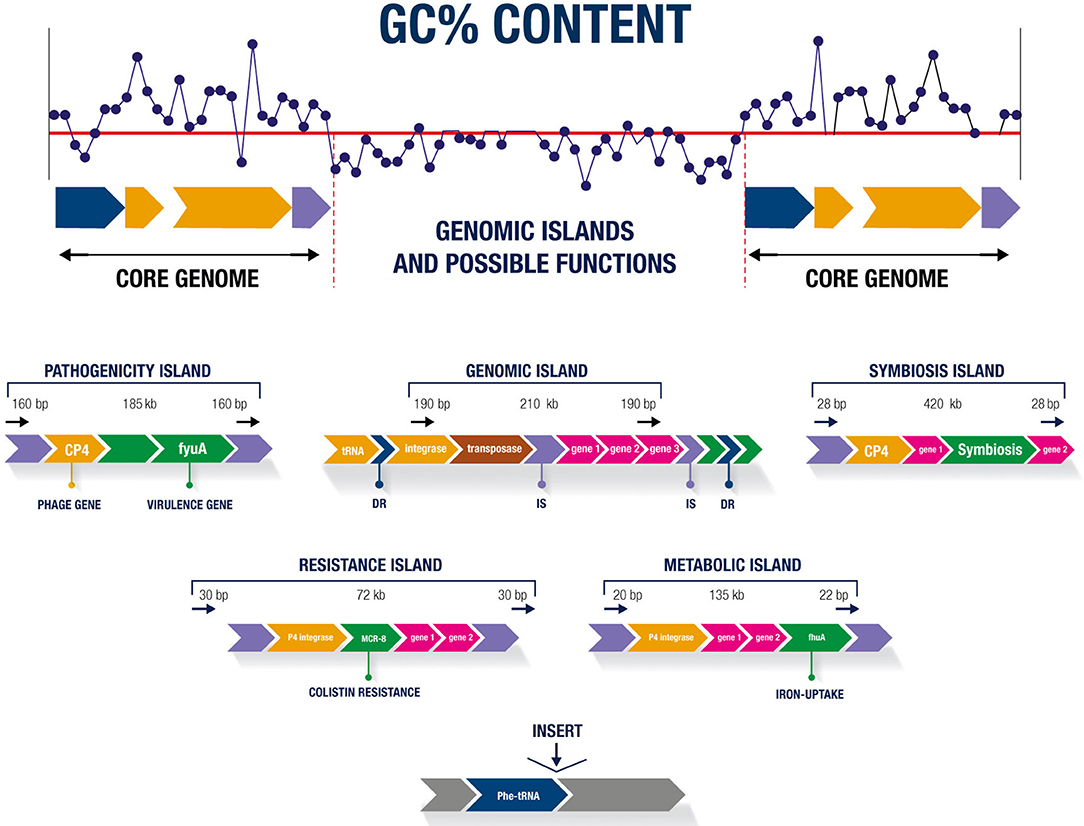
\includegraphics[width=0.8\linewidth]{images/ilot_genomique.jpg}
    \caption[Îlots génomiques et leur caractéristique]{\textbf{Îlots génomiques et leur caractéristique.} Extrait de  \cite{da_silva_filho_comparative_2018}}
    \label{fig:GI}
\end{figure}

\newpage
Ces GIs sont complexes à étudier, car ils concentrent les variations, même entre génomes proches. L'histoire évolutive est souvent difficile à reconstituer, tant des éléments ont été intégrés et éliminés au cours du temps (\autoref{fig:cycle_IG}). En plus de s'échanger avec d'autres organismes \cite{buchrieser_high-pathogenicity_1998}, les GIs peuvent se déplacer au sein du génome \cite{karaolis_bacteriophage_1999}.

\begin{figure}[htbp]
    \centering
    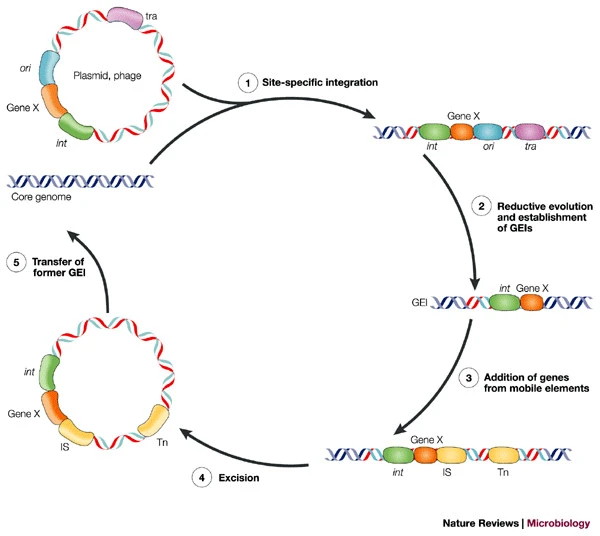
\includegraphics[width=0.65\linewidth]{images/cycle_GI.png}
    \caption[Cycle de vie d'un îlot génomique]{Cycle de vie d'un îlot génomique. Extrait de \cite{dobrindt_genomic_2004}}
    \label{fig:cycle_IG}
\end{figure}

Les GIs ne s'insèrent pas n'importe où dans les génomes. On les retrouve fréquemment dans des zones où de nombreux éléments se sont insérés au cours de l'évolution d'un taxon. Ces régions sont appelées : point chaud d'insertion (\textit{hotspot} en anglais).
À l'intérieur des \textit{hotspots}, on retrouve une grande variabilité du contenu génique entre les génomes. Les \textit{hotspots} sont également caractérisés par des bordures composées de gènes communs à l'ensemble des génomes. 

Ils présentent également une recombinaison homologue accrue dans les gènes flanquant les \textit{hotspots}, avec 50 \% d’événements de recombinaison et 30 \% d’incongruence phylogénétique\footnote{L'incongruence phylogénétique désigne une discordance entre l’arbre phylogénétique d’un gène spécifique et l’arbre phylogénétique global construit à partir d'un grand nombre de gènes conservés.} par rapport à l'arbre des espèces. Ces \textit{hotspots} contiennent 50 \% des gènes acquis par HGT \cite{oliveira_chromosomal_2017}. Ils sont enrichis en gènes liés à la motilité, à la défense, à la transcription, à la réplication et à la réparation de l’ADN \cite{flores_ramos_genomic_2021}.

Le contenu génique du \textit{hotspot} provient d'une accumulation progressive de gènes, comme le suggère le faible pourcentage (8 \%) de \textit{hotspots} composés uniquement de gènes spécifiques à une souche \cite{oliveira_chromosomal_2017}. Cette accumulation peut se faire par bloc de gènes. Ces blocs, conservés dans le \textit{hotspot}, sont appelés modules \cite{lescat_module_2009}. Cette modularité pourrait expliquer l'organisation complexe des îlots génomiques \cite{touchon_organised_2009}.
Les \textit{hotspots} sont donc communs à un groupe d'organismes, et définis au niveau d'un taxon. Il est donc nécessaire de mener des études de comparaison des génomes pour les identifier.